\chapter{Compressive Sensing}
\label{ch:cs}

% \emph{
% \begin{itemize}
% \item Problem Statement for discrete. Img, Vids as unrolled vec. Sparsity -> Compression (adaptive). Why wasteful.
% \item CS is NON-ADAPTIVE. Sensing Matrix. Much fewer measurements.
% \item Against Fund Thm of LA -> resolve by sparsity (show a graphic).
% \item What Sensing matrix? We've only done masks, so maybe no point in talking about RIP etc -> just reference.
% \item Signal Recovery. L2 vs L0 vs L1 + Geometry?.
% \item We focus on Reconstruction. Side note to single-px cam (in \@ sensing). Perhaps this should go in Ch1:Background
% \item Bayesian CS (or put it in Ch5?)
% \end{itemize}
% }

% \emph{
%   \begin{enumerate}
%   \item Conventional DSP + Promise of CS
%   \item CS Problem
%   \item CS Solution Strategy
%     \begin{enumerate}
%     \item Sparsity
%     \item Incoherence
%     \end{enumerate}
%   \item CS Reconstruction
%   \end{enumerate}
% }


In this chapter we will outline the main ideas of the \emph{Compressive Sensing} framework (also known as \emph{Compressed Sensing, Compressed Sampling, Compressive Samping} or \emph{CS}).
We begin by discussing conventional approaches to data acquisition and compression, and how CS differs from that.
Next, formulate the CS Problem.
Following that, we briefly discuss the general solution strategy.
Lastly, give a brief overview of deterministic approaches to CS reconstruction (maybe).

In Chapter \ref{ch:msce}, we will discuss a Bayesian approach to solving the Compressive Sensing Problem.


\section{Signal Acquisition and Compression}
\subsection{Acquisition}
In order to work with information within analog signals (continuous streams of data) such as sounds, images or video, we rely on reducing the analog signals to digital (discrete) signals that can be processed with computers.
This digitization is done by taking discrete measurements of the analog signal at certain points in time or space, a process known as \emph{sampling}.

Conventional approaches to sampling are based on the \emph{Shannon/Nyquist Sampling Theorem} \cite{shannon1949}:
When sampling a band-limited signal uniformly, we are able to \emph{perfectly reconstruct} the signal from its samples if the sampling rate is at least twice the bandwidth of the signal.

We briefly illustrate this in Figure \ref{fig:nyquist}.
Consider an analog signal $x(t)$ that varies with time, such as an audio wave.
Let $f$ be the highest frequency present in $x(t)$.

In order to digitise $x(t)$, we measure $x$ at discrete points in time $t^{(0)}, \cdots, t^{(n)}$ and store the samples $x^{(i)} \equiv x(t^{(i)})$.
We sample $x$ uniformly, measuring a sample every $T_s$ seconds, so that $t^{(i)} = iT_s$.
The sampling rate is therefore $f_s = 1/T_s$.

\begin{figure}
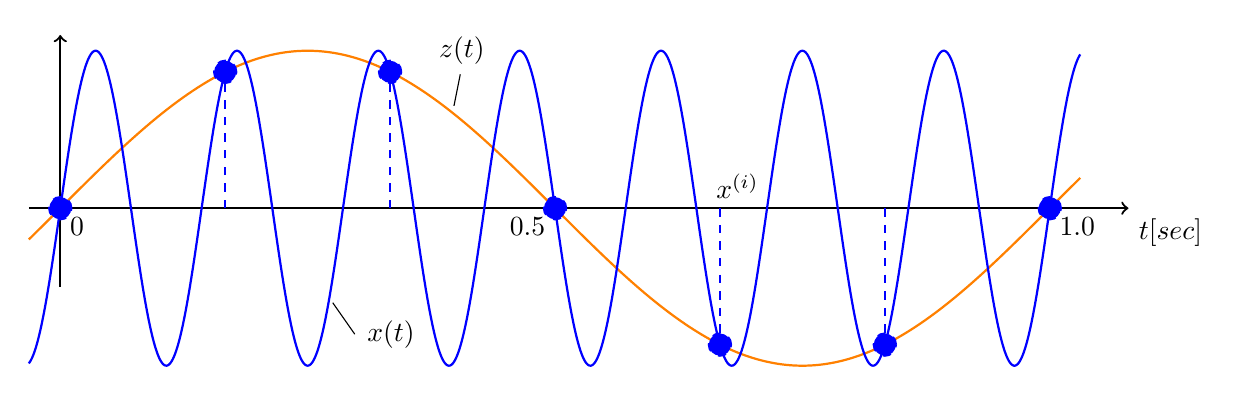
\begin{tikzpicture}[scale=2]
  \draw [thick,->](-0.2,0) -- (2*pi+0.5,0) node[below right] {$t [sec]$};
  \draw [thick,->](0,-0.5) -- (0,1.1);
  \draw [domain=-0.2:2*pi+0.2,samples=1000,orange, thick] plot(\x,{sin(\x r)});
  \draw [domain=-0.2:2*pi+0.2,samples=1000,blue, thick] plot(\x,{sin(7*\x r)});  
  \draw [domain=0:2*pi, samples=7, ycomb, mark=*,blue, dashed, thick] plot(\x,{sin(\x r)});
  \node at (2.55,1) {$z(t)$};
  \draw (2.54,0.85) -- (2.5,0.65);
  \node at (2.1,-0.8) {$x(t)$};
  \draw (1.87,-0.8) -- (1.73,-0.6);
  \node at (4.3,0) [above] {$x^{(i)}$};
  \node at (2*pi,0) [below right] {$1.0$};
  \node at (pi,0) [below left] {$0.5$};
  \node at (0,0) [below right] {$0$};
\end{tikzpicture}
\caption[Illustration of Nyquist Sampling]{Illustration of the Shannon/Nyquist Sampling Theorem. The orange curve is the original signal $x(t)$ which is a sinusoid with frequency $f = 7$ Hz. The blue points are discrete samples $x^{(i)}$ taken from $x(t)$ at a sampling rate $f_s = 7$ Hz, which is below the Nyquist Rate $2f = 14$ Hz. Thus, aliasing occurs and interpolation algorithms will reconstruct an alias $z(t)$ of $x(t)$.}
\label{fig:nyquist}
\end{figure}

Suppose we wish to reconstruct $x(t)$ by interpolating the samples.
There is an infinite number of continuous functions that fit this set of samples.
However, it can be shown that only one of them has a bandwidth of no more than $f_s/2$.
Thus, if $f < f_s/2$ (the \emph{Nyquist Criterion}), then $x(t)$ is the unique function that will be approximated by interpolation algorithm such as the \emph{Whittaker-Shannon interpolation formula}\cite{shannon1949}.

In Figure \ref{fig:nyquist}, we have a sinusoidal signal $x(t)$ with frequency $f$.
The sampling rate is $f_s=f$ and therefore below the signal's \emph{Nyquist rate} $2f$. 
Thus, we are unable to reconstruct $x(t)$ from the samples. 
Instead, we will reconstruct an \emph{alias} $z(t)$ which, in this case, is another sinusoid with frequency $f/7$.
The original signal $x$ is lost.

We have illustrated Nyquist sampling in the 1-dimensional case.
The same principles hold for higher dimensional signals such as images and videos.

For signals that vary with space, the sampling rate is governed by the desired spatial resolution.
In order to recover the finer details (the high-frequency components) of an image, we require higher pixel density (i.e. more pixels per 

Nyquist sampling underlies almost all signal acquisition protocols that are found in practice. 
It is the basis of medical imaging devices, consumer electronics such as audio and video recorders, radio receivers, etc.

\subsection{Compression}
The sampling theorem imposes a lower bound on the sampling rate above which we get are able to perfectly reconstruct the desired signal.
This lower bound is often very high and we end up with a very large number of measurements.
Storage and transfer of such signals becomes prohibitavely expensive as the size of the signal grows.
Thus, a need for \emph{data compression} arises.

We will discuss a particular type data compression known as \emph{transform coding}.
It is the standard compression method for ``natural'' and manmade signals such as audio, photos, and video and is the basis of many common signal formats such as JPEG for images, MPEG for videos and MP3 for audio.

Let $\bm v$ by a real-valued digital signal of length $M$, $\bm v \in \mathbb{R}^M$.
Without loss of generality, $\bm v$ is assumed to be a one-dimensional signals.
If we are working with a multi-dimensional signals, we may first vectorize it into a long vector.
When compressing digital signals, we are usually interested in \emph{lossy compression}.

Any vector in $\mathbb{R}^M$ can be expressed as a linear combination of $M$ \emph{basis vectors} $\bm\psi_j \in \mathbb{R}^M$:
\begin{equation}
\label{eqn:cs-transform1}
  \bm v = \sum_{j=1}^M w_j \bm\psi_j
\end{equation}
where $w_j$ is the coefficient (or weight) associated with $\bm\psi_j$.

By forming the \emph{basis matrix} $\bm\Psi = \left[\bm\psi_1 \,\cdots\, \bm\psi_M\right]$, we can express equation (\ref{eqn:cs-transform1}) in matrix form
\begin{equation*}
\bm v = \bm\Psi \bm w
\end{equation*}
where $\bm w = (w_1,\cdots,w_M)^T$.
For simplicity, we assume that the basis $\bm\Psi$ is orthonormal, so that $\bm\Psi\bm\Psi^T = \bm I_M$ and $\bm\psi_i^T\bm\psi_j$ is 1 if $i = j$ and 0 otherwise.
Thus, the coefficient $w_j$ is given by $w_j = \bm v^T\bm\psi_j$.

We now have two equivalent representations of the same signal, $\bm v$ in the original basis and $\bm w$ in the $\bm\Psi$ basis.
Since $\bm\Psi$ is orthogonal, $\bm v$ and $\bm w$ have the same $\ell_2$-norm, $||\bm v||_2 = ||\bm\Psi\bm w||_2 = ||\bm w||_2$.

While in the original signal $\bm v$ the energy is spread over many of its components, it is possible to find a basis $\bm\Psi$ such that the energy of the transformed signal $\bm w$ is concentrated in only a few large components $w_j$.
Thus a large fraction of the entries in $\bm w$ are very close to zero.

Suppose that we delete the entries $w_j$ that are very small and replace them with zero to obtain $\bm{\hat w}$.
Let $\bm{\hat v} = \bm\Psi\hat{\bm w}$ the approximate signal in the original domain.
Since $\bm{\hat w}$ is very close to $\bm w$, so that $||\bm{\hat w} - \bm w||_2$ is very small, it follows that
\begin{equation*}
  ||\bm{\hat v} - \bm v||_2 = ||\Psi\bm{\hat w} - \Psi\bm w||_2 = ||\Psi (\bm{\hat w} - \bm w||_2 = ||\bm{\hat w} - \bm w)||_2
\end{equation*}
is also very small.

\begin{figure}
  \centering
  \begin{subfigure}[b]{0.4\textwidth}
    \includegraphics[width=\textwidth]{Chapter2/Images/lenna512.png}
    \caption{Uncompressed Image}
    \label{fig:ch2:lenna_orig}
  \end{subfigure}
  \begin{subfigure}[b]{0.4\textwidth}
    \includegraphics[width=\textwidth]{Chapter2/Images/lenna512_dct.png}
    \caption{Compressed Image via DCT}
    \label{fig:ch2:lenna_dct}
  \end{subfigure}
  \caption[Image Compression using DCT]{The uncompressed image has a resolution of $512\times 512$, i.e. 262144 pixels. We compress the image by performing a Discrete Cosine Transform and storing only the largest 27832 coefficients. The compression ratio is 9.42.}
  \label{fig:ch2:dct}
\end{figure}

Thus, a viable method for lossy compression of the signal $\bm v \in \mathbb{R}^M$ would be the following:
\begin{enumerate}
\item Compute the full set of transform coefficients $\{w_j\}_{j=1}^M$ via $\bm w = \Psi^T\bm v$.
\item Locate all the coefficients $w_j$ whose absolute value is above a certain threshold (suppose there are $K$ of them). 
\item Discard all the $(M-K)$ small coefficients
\item Store the values and locations of the $K$ large coefficients
\end{enumerate}
It is possible to find basis matrices $\bm\Psi$ that result in very high compression ratios for a wide range of natural signals without any noticable reduction in the signal quality.
Furthermore, many of the commonly used basis transforms can be computed very efficiently.

Audio signals and a wide class of communication signals are highly compressible in the localized Fourier basis.
Images and video signals are often compressed via the \emph{Discrete Cosine Transform} (DCT) or the \emph{Discrete Wavelet Transform} (DWT).
For instance, the JPEG standard for image compression is based on the DCT, while the more modern JPEG2000 format uses the CDF 9/7 wavelet transform or the CDF 5/3 wavelet transform \cite{taubman2012}.

In Figure \ref{fig:ch2:dct}, we compress the standard test image ``Lenna'' via a DCT. 
We are only storing about 10\% of the transform coefficients.
Yet, the difference between the original image and the compressed image is hardly noticable.

We will discuss the DCT and the DWT in more detail in Chapter \ref{ch:dwt}.

\subsection{A Novel Approach: Compressed Sampling}
Circumvent Shannon by non-uniform sampling or by using alternative sampling matrices.


\section{The Compressive Sensing Problem}



This section is based on \cite{pilikos2014}. 
The problem to be solved can be formulated as follows: Let $\bs x \in \mathbb{R}^N$ be a signal of interest.
We do not measure $\bs x$ directly and it is thus unknown.
Instead, we have a measurement $\bs y \in \mathbb{R}^M$, with $M << N$, from which we want to reconstruct $\bs x$.
The signals $\bs x$ and $\bs y$ are related as follows:
\begin{equation}
\label{eqn:CS}
\bs \Omega \bs x = \bs y
\end{equation}
where $\bs \Omega$ is a known $M\times N$ matrix referred to as the \emph{sensing matrix}.

For example, in \cite{pilikos2014}, the signal of interest $\bs x$ is an image, so that $N$ is equal to the total number of pixels in the image and $x_i$ is equal to the intensity of the corresponding pixel.
However, we imagine that we have only access to a corrupted version of $\bs x$ in which random pixel values have been deleted.
This is our measurement $\bs y$.
The sensing matrix $\bs\Omega$ corresponding to this scenario is obtained by taking the $N\times N$ identity matrix and deleting the rows that correspond to the missing entries in $\bs x$.

Compressive Sensing (CS) is a collection of signal processing techniques that allow for efficient \emph{reconstruction} (and indeed \emph{aquisition}) of such signals by solving the underdetermined system (\ref{eqn:CS}).

Of course, there are infinitely many solutions to an underdetermined system.
In the CS framework, we seek to find a solution $\hat{\bs x}$ that is \emph{sparsest in some domain}.
By that, we mean that we want to find $\hat{\bs x}$ that satisfies (\ref{eqn:CS}), such that there exists a basis transformation of $\hat{\bs x}$ in which it has the smallest number of nonzero entries.

More concretely, we assume there exists a domain in which the desired signal $\bs x$ is sparse. 
I.e. there exists a $N\times N$ basis matrix $\Psi$ such that $\bs x = \bs\Psi \bs w$ and $\bs w$ is sparse.

The CS problem can then be expressed as follows:
\begin{equation}
\label{eqn:CSproblem}
\min||\bs w||_0 \qquad\mbox{subject to}\qquad \bs\Omega\bs\Psi\bs w = \bs y
\end{equation}
where $||.||$ denotes the $l_0$ norm, i.e. the number of nonzero components.


\section{The Solution}
\subsection{Stable Measurement Matrix}
\emph{Matrices}
\subsection{Reconstruction Algorithms}
\emph{L0, L1, L2, Deterministic, Geometry}

For a more detailed review of the CS framework, see \cite{candes2008}.

